\documentclass[letterpaper,10pt,conference]{ieeeconf}

\IEEEoverridecommandlockouts
\overrideIEEEmargins

\usepackage{amsmath,amssymb}
\usepackage{booktabs}
\usepackage{graphicx}
\usepackage{xcolor}
\usepackage{url}

\newcommand{\method}{\textsc{CalibAgent}}
\newcommand{\vect}[1]{\boldsymbol{#1}}

\title{CalibAgent: Task-Aware Active Calibration and Shift Recovery\\
for Quadruped Velocity Commands}

\author{Anonymous Authors}

\begin{document}
\maketitle
\thispagestyle{empty}
\pagestyle{empty}

\begin{abstract}
Commercial and learned quadruped controllers often expose a planar velocity
command while hiding the dynamics that map commands to realized motion.
Payload, surface, controller, and estimator changes can therefore preserve
balance yet distort navigation. We present \method, an active calibration layer
for this opaque interface. A Bayesian command-to-motion model represents
cross-axis coupling and asymmetric response; a task-weighted integrated
variance objective selects informative commands for the intended deployment
distribution. Hard safety checks, validation-based stopping, constrained
inverse compensation, and residual-triggered recovery remain separate from the
learned acquisition score. On 183 passive Unitree Go2 trials, a coupled affine
model reduces held-out velocity RMSE by 54.5\% relative to raw commands. In
registered synthetic experiments, task weighting reaches joint accuracy and
uncertainty targets in 18.67 trials, saving 39.5\% against Latin hypercube
sampling and 18.8\% against D-optimal design. Pinned Isaac Lab experiments show
9.3--31.7\% held-out RMSE reduction, faster early recovery under four shifts,
and successful budgeted navigation across six prospectively frozen maps. These
results establish the calibration and recovery mechanism under the registered
conditions; active hardware calibration and navigation are reserved for the
planned real-robot study.
\end{abstract}

\section{Introduction}

A quadruped can remain upright while executing the wrong motion. High-level
controllers accept a desired planar velocity
$\vect{u}=[v_x,v_y,\omega_z]^\top$, but the steady body velocity may contain
gain error, dead zones, saturation, and cross-axis coupling. These errors are
particularly consequential when a planner assumes that the exposed command is
a calibrated control variable. Taouil \emph{et al.} showed that learned motion
models of a black-box quadruped controller can improve footstep planning
\cite{taouil2023blackbox}; related work has calibrated velocity-controlled
kinematic models online for wheeled visual--inertial odometry
\cite{li2022vio}. The remaining question is how to collect the calibration
trials themselves when hardware time is limited and the useful part of command
space is task dependent.

Robot calibration has long treated measurement configuration as a design
variable \cite{hollerbach1996calibration,calafiore2001dynamic}. Classical
observability and D-optimal criteria prioritize parameter identification
\cite{sun2008observability,sun2008active}. Task-oriented calibration instead
scores a design by uncertainty at the end-effector or another quantity of
interest \cite{carrillo2013task,attia2018goal}. We apply that principle to the
external velocity interface of a fixed quadruped controller: trials are chosen
for their reduction of predictive uncertainty over commands expected during
deployment, not for uniform parameter-space coverage.

This layer differs from locomotion-policy adaptation. RMA conditions a trained
policy on latent environment estimates \cite{kumar2021rma}, residual models can
update model-based legged controllers online \cite{sun2021unknown}, and recent
embodiment adaptation identifies hardware changes from short interaction
histories \cite{li2026embodiment}. \method\ neither retrains nor instruments the
low-level controller. It identifies the mapping from user commands to measured
steady motion, translates desired velocities through a constrained inverse, and
reactivates calibration when predictive residuals indicate a shift.

This paper makes four contributions. First, it formulates the opaque
command-to-motion interface as a compact Bayesian regression with coupled,
asymmetric features and per-trial measurement uncertainty. Second, it derives
an exact task-weighted integrated variance reduction (IVR) score for sequential
command selection. Third, it separates statistical learning from hard safety,
validated stopping, and bounded shift recovery. Fourth, it evaluates the chain
from model need to downstream navigation using passive Go2 data, controlled
synthetic families, fault injection, pinned physics simulation, and a retained
failed confirmation followed by a disjoint prospective replication. The
current hardware evidence is passive; real online calibration, shift recovery,
and navigation remain outside the reported results.

\begin{figure*}[t]
  \centering
  \setlength{\tabcolsep}{2pt}
  \begin{tabular}{@{}ccc@{}}
    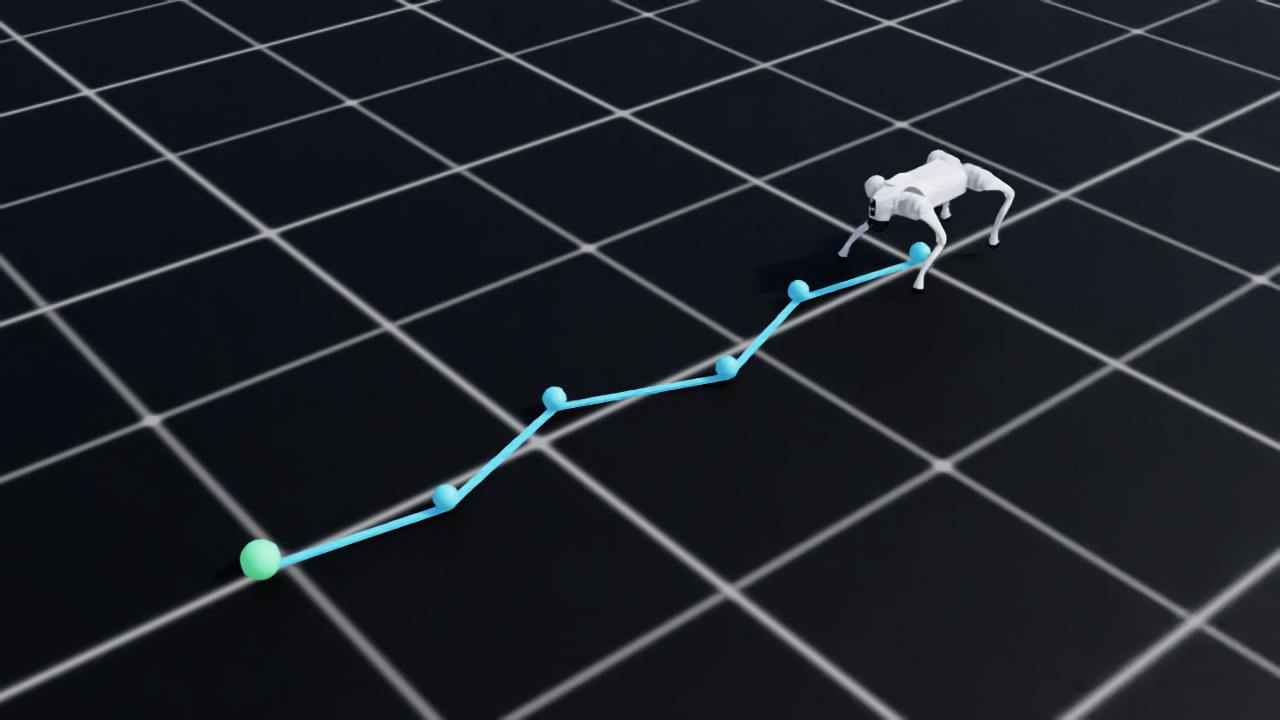
\includegraphics[width=0.318\textwidth]{../docs/assets/readme/isaac_sim/p7_replicate_s_bend_overview.png} &
    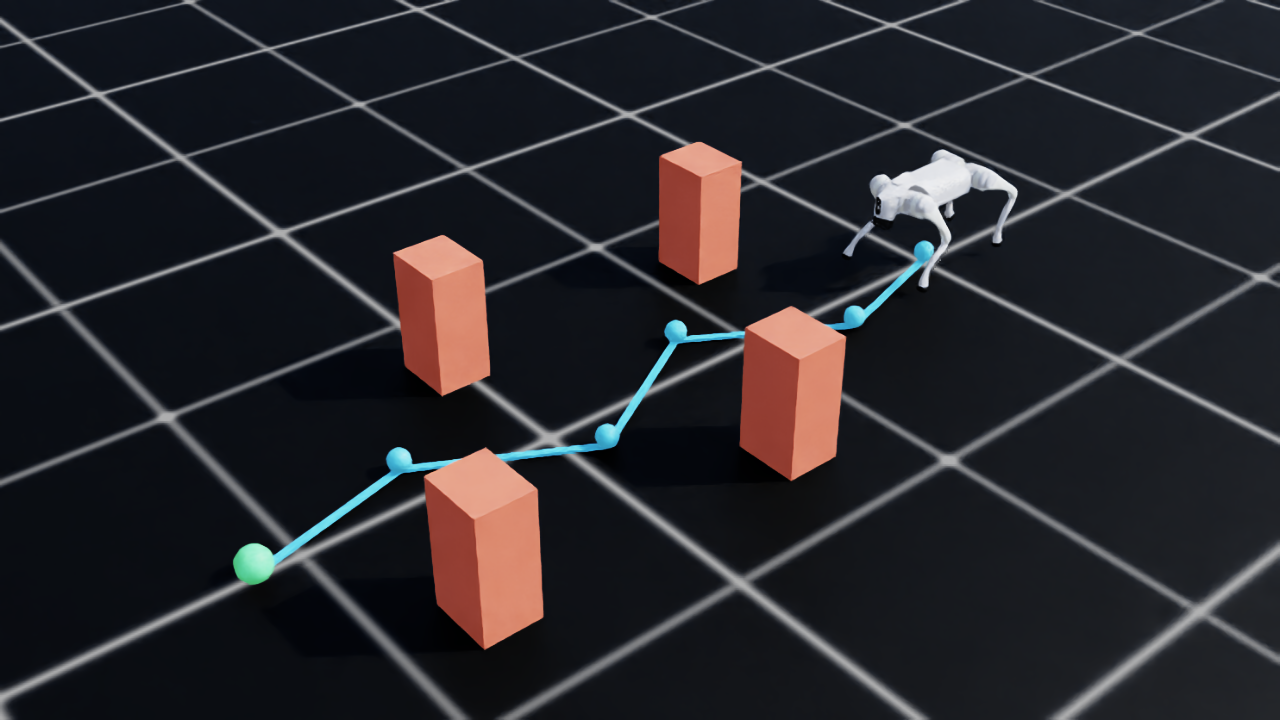
\includegraphics[width=0.318\textwidth]{../docs/assets/readme/isaac_sim/p7_replicate_offset_slalom_overview.png} &
    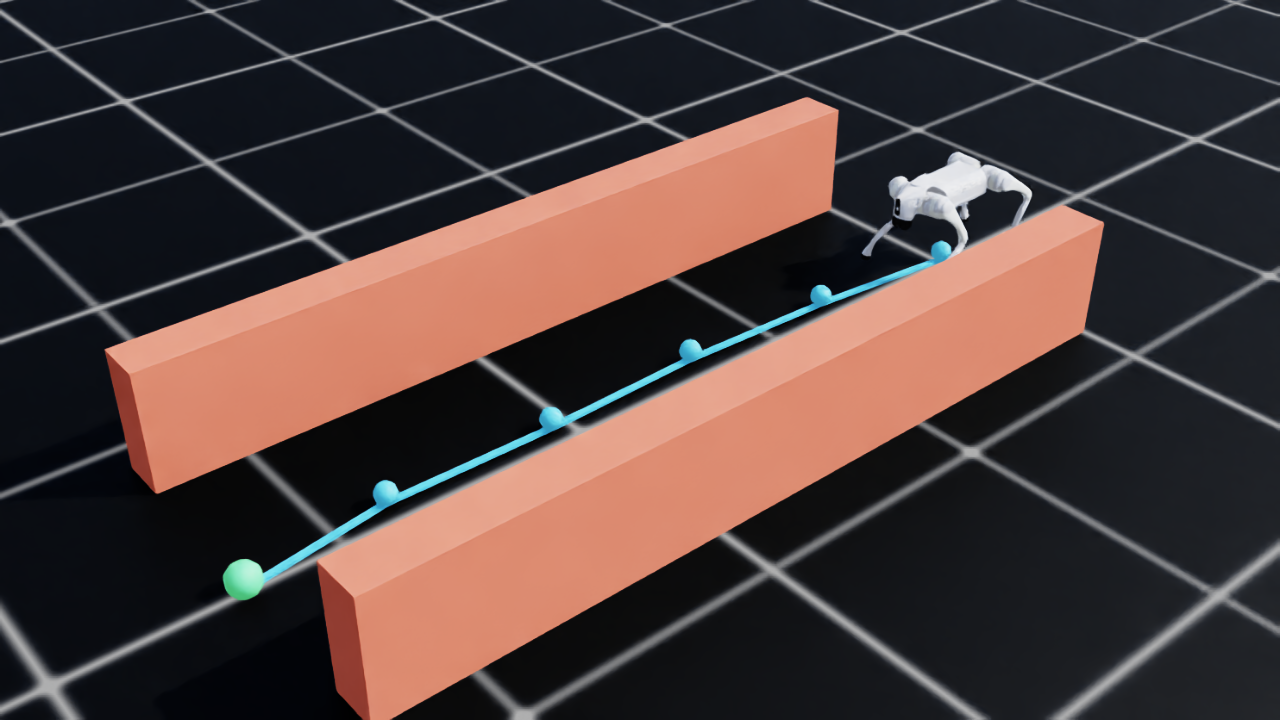
\includegraphics[width=0.318\textwidth]{../docs/assets/readme/isaac_sim/p7_replicate_narrow_lane_overview.png} \\
    \textbf{(a) S-bend} & \textbf{(b) Offset slalom} & \textbf{(c) Narrow lane} \\[2pt]
    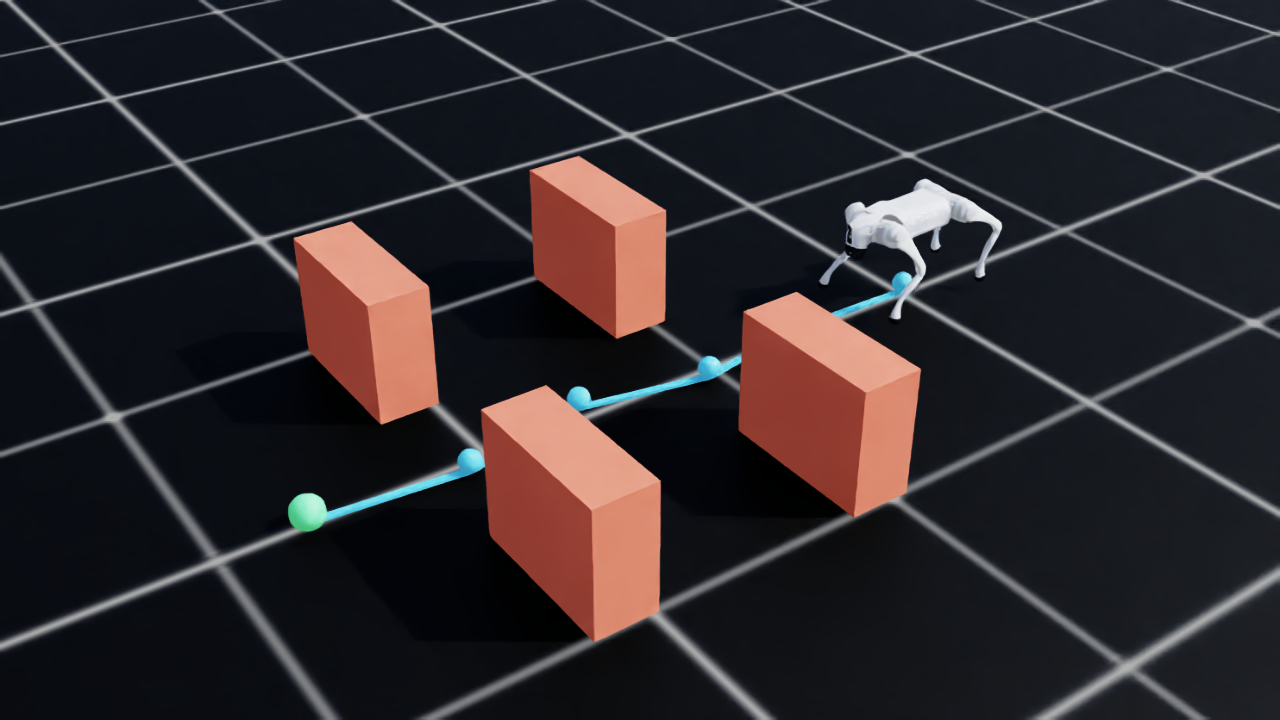
\includegraphics[width=0.318\textwidth]{../docs/assets/readme/isaac_sim/p7_replicate_double_chicane_overview.png} &
    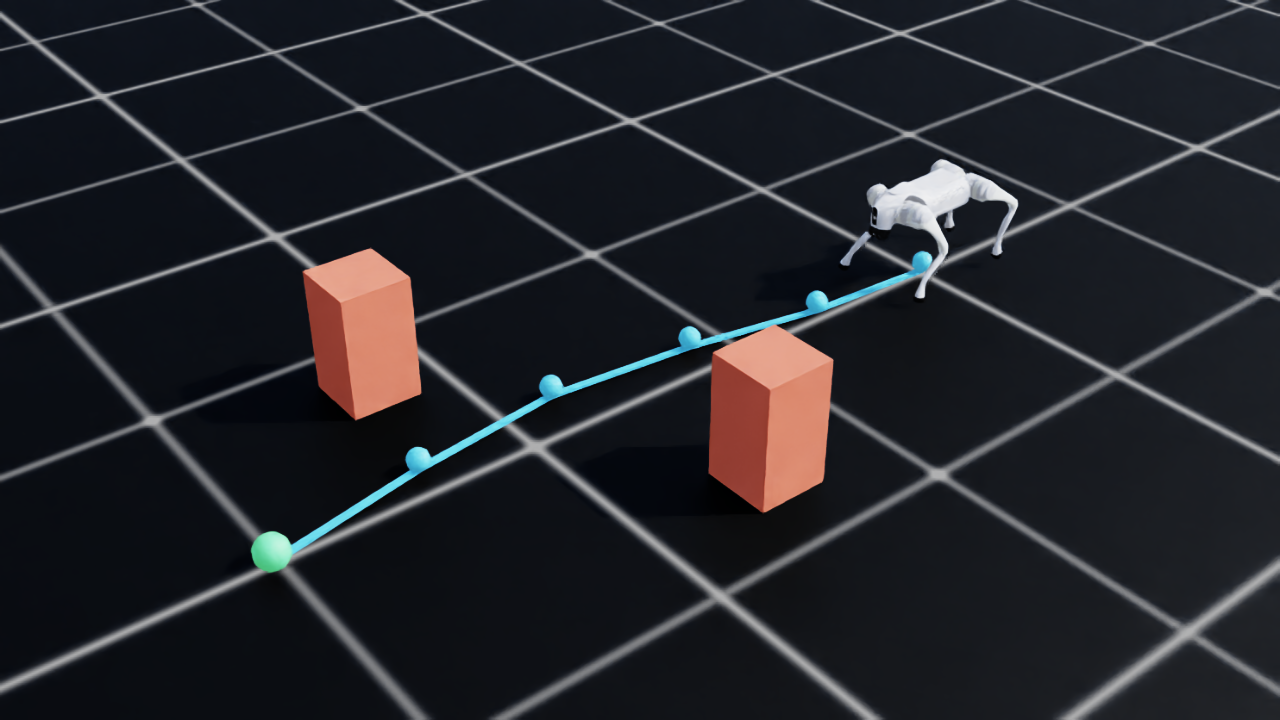
\includegraphics[width=0.318\textwidth]{../docs/assets/readme/isaac_sim/p7_replicate_weighted_arc_overview.png} &
    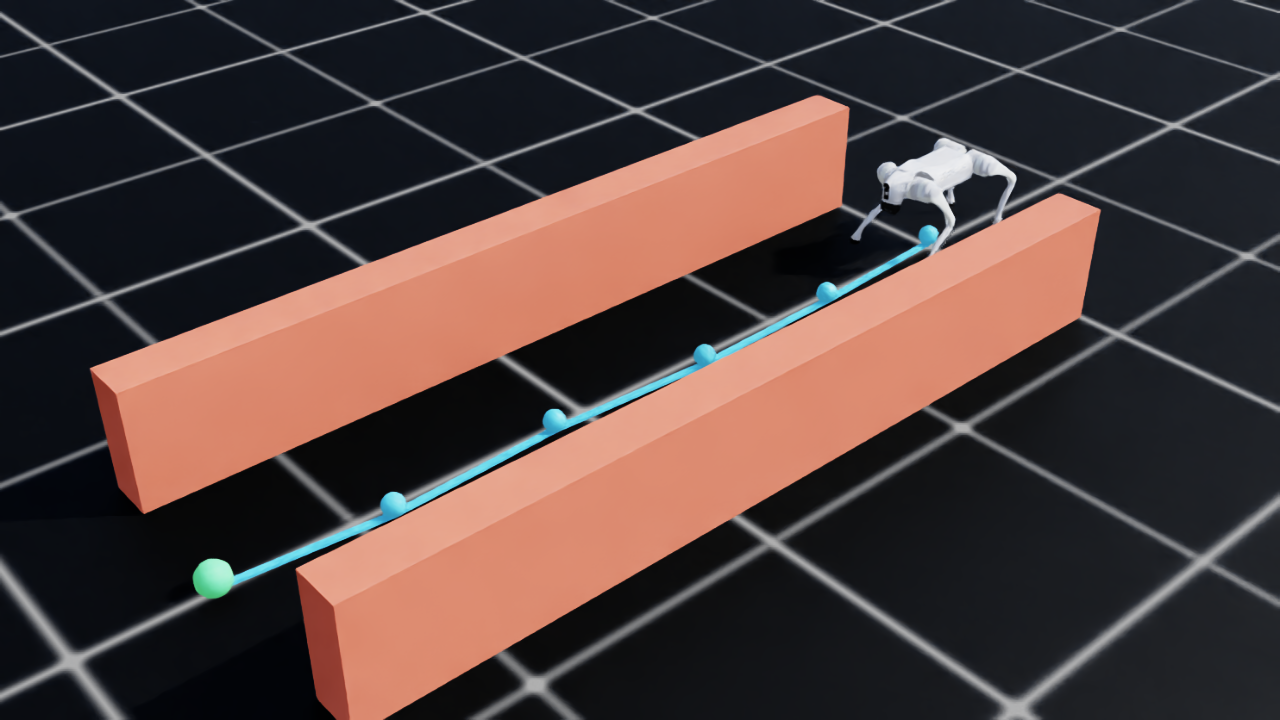
\includegraphics[width=0.318\textwidth]{../docs/assets/readme/isaac_sim/p7_replicate_extended_lane_overview.png} \\
    \textbf{(d) Double chicane} & \textbf{(e) Weighted arc} & \textbf{(f) Extended lane}
  \end{tabular}
  \caption{Elevated Isaac Sim views of all six frozen P7 prospective-replication
  maps. Cyan segments and spheres reproduce the map waypoints; orange geometry
  reproduces the registered obstacles. The overlays are non-colliding
  visualization geometry and do not contribute to the quantitative endpoints.}
  \label{fig:p7maps}
\end{figure*}

\section{Related Work}

\subsection{Calibration and Experimental Design}

Kinematic and dynamic robot calibration depend on both model structure and the
poses or trajectories used for identification
\cite{hollerbach1996calibration,calafiore2001dynamic}. Sun and Hollerbach linked
robot observability indices to alphabetic optimal design and developed an
efficient active pose-selection algorithm
\cite{sun2008observability,sun2008active}. Carrillo \emph{et al.} then selected
configurations by predicted task-space error rather than only parameter
covariance \cite{carrillo2013task}. This task-space view parallels
goal-oriented Bayesian design, which minimizes uncertainty in a downstream
quantity of interest \cite{attia2018goal}. Greedy information selection also
has established connections to near-optimal sensor placement
\cite{krause2008sensor}. \method\ uses a related predictive objective, but its
design variable is a safety-filtered velocity command and its quantity of
interest is the realized velocity over a frozen deployment distribution.

\subsection{Legged Command Models and Adaptation}

Simulation-trained policies have produced agile and terrain-robust quadruped
locomotion \cite{hwangbo2019agile,lee2020terrain,rudin2022minutes}. Robust
locomotion, however, does not make the user-level velocity interface exact.
Learned black-box motion models can bridge that interface for planning
\cite{taouil2023blackbox}, while steady-state and local dynamics models can
adapt a legged robot to unmodeled disturbances \cite{fey2024adapt}. Policy-level
adaptation and domain randomization address broader changes
\cite{kumar2021rma,curtis2025flow,li2026embodiment}. \method\ occupies a narrower
operational layer: it actively calibrates a fixed controller's command response,
quantifies posterior uncertainty, and applies compensation only inside a
non-learned envelope.

\section{Method}

\begin{figure*}[t]
  \centering
  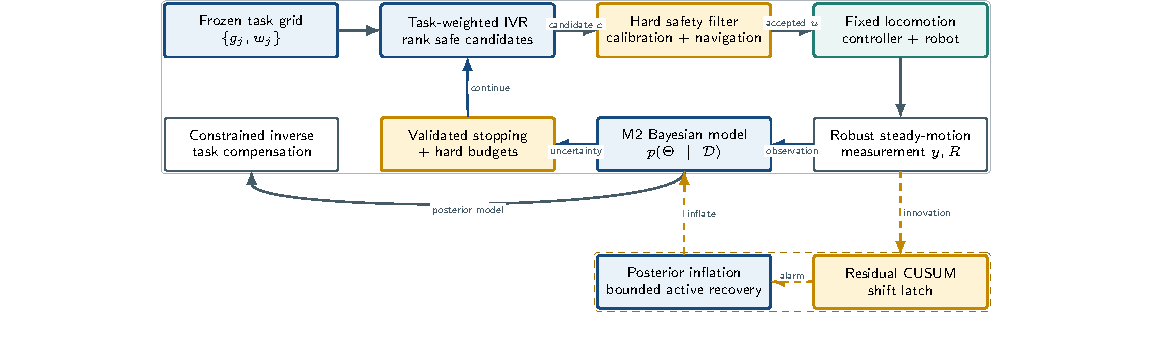
\includegraphics[width=0.98\textwidth]{figures/calibagent_pipeline.pdf}
  \caption{\method\ architecture. Task-weighted acquisition ranks calibration
  commands, but the hard filter alone authorizes execution. Valid observations
  update the Bayesian model; held-out validation and uncertainty control
  stopping. A latched residual alarm inflates posterior uncertainty and opens a
  bounded active-recovery phase. The inverse compensator uses the same bounded
  command set during navigation.}
  \label{fig:pipeline}
\end{figure*}

Figure~\ref{fig:pipeline} separates the probabilistic calibration loop from the
rules that constrain its operation. The low-level locomotion controller is
fixed and treated as a black box. A trial executes a constant body-frame
command after warm-up and ramp-in, extracts a robust steady-motion observation,
and records its covariance and validity. Invalid observations never update the
posterior.

\subsection{Bayesian Command-to-Motion Model}

Let $\vect{y}\in\mathbb{R}^3$ denote the measured steady velocity for command
$\vect{u}$. A fixed basis $\vect{\phi}(\vect{u})$ contains an intercept, the
three command axes, pairwise products, and positive/negative hinge terms for
each axis. The affine M1 variant uses only the intercept and command axes; M2
adds the coupled and hinge features. Feature statistics are fitted once on a
predeclared command reference, never on held-out outcomes.

For output axis $a$, the model is
\begin{equation}
 y_a=\vect{\theta}_a^\top\vect{\phi}(\vect{u})+\epsilon_a,
 \quad
 \epsilon_a\sim\mathcal{N}(0,\sigma_a^2+r_a),
 \label{eq:model}
\end{equation}
where $r_a$ is the observation covariance diagonal. Given prior
$\mathcal{N}(\vect{m}_{a0},\vect{\Sigma}_{a0})$, sequential updates use
\begin{align}
 \vect{\Lambda}_a &\leftarrow \vect{\Lambda}_a+
 \frac{\vect{\phi}\vect{\phi}^\top}{\sigma_a^2+r_a}, \\
 \vect{\eta}_a &\leftarrow \vect{\eta}_a+
 \frac{\vect{\phi}y_a}{\sigma_a^2+r_a},
 \quad
 \vect{\Sigma}_a=\vect{\Lambda}_a^{-1},\quad
 \vect{m}_a=\vect{\Sigma}_a\vect{\eta}_a .
 \label{eq:update}
\end{align}
The predictive mean is $\mu_a(\vect{u})=\vect{m}_a^\top\vect{\phi}(\vect{u})$,
and the predictive variance is
$\vect{\phi}^\top\vect{\Sigma}_a\vect{\phi}+\sigma_a^2$. Independent output
posteriors keep the online update small while coupled input features represent
cross-axis response.

\subsection{Task-Weighted Active Selection}

A frozen task distribution is represented by grid commands
$\{\vect{g}_j\}_{j=1}^{G}$ and normalized weights $w_j$. For candidate
$\vect{c}$, the posterior covariance update is independent of the unknown
outcome. The exact reduction in weighted epistemic variance is therefore
\begin{equation}
 \mathcal{I}(\vect{c})=
 \sum_{a=1}^{3}\sum_{j=1}^{G} w_j
 \frac{\left(\vect{\phi}(\vect{g}_j)^\top\vect{\Sigma}_a
 \vect{\phi}(\vect{c})\right)^2}
 {\sigma_a^2+\vect{\phi}(\vect{c})^\top\vect{\Sigma}_a
 \vect{\phi}(\vect{c})}.
 \label{eq:ivr}
\end{equation}
The planner maximizes $\mathcal{I}(\vect{c})-\lambda_r R(\vect{c})-
\lambda_d D(\vect{c})$ over a finite command pool after excluding commands too
close to prior trials. Greedy batches use covariance-only fantasy updates, so
no unobserved target is imputed. The registered main planner uses 512
candidates, an eight-command seed design, a 400-point task grid, and a 0.025
normalized duplicate radius.

\subsection{Safety, Stopping, Compensation, and Shift Recovery}

The hard filter checks finite state, localization, battery, roll, pitch, base
height, command bounds, linear norm, coupled linear--angular load, command slew,
and projected workspace occupancy. It evaluates ranked candidates after
planning and fails closed when none remains. A 50~Hz monitor can zero the
command independently of the planner. This separation prevents uncertainty
reduction from trading against a learned safety penalty.

Stopping requires minimum trial coverage and held-out validation. A run stops
at the registered target only after three consecutive confirmations of both
validation RMSE and integrated uncertainty; a low-gain condition also requires
valid held-out accuracy. Trial, time, distance, and battery budgets take
priority. For deployment, the inverse compensator searches the same bounded
candidate set and minimizes
\begin{equation}
 \|\vect{\mu}(\vect{u})-\vect{v}^{*}\|_2^2+\lambda
 \|\vect{u}-\vect{v}^{*}\|_2^2+\rho\sum_a s_a^2(\vect{u}),
 \label{eq:inverse}
\end{equation}
then passes the selected command through the hard filter.

Shift detection uses normalized innovation energy
$z_t=\vect{e}_t^\top\vect{S}_t^{-1}\vect{e}_t/3$. A one-sided CUSUM accumulates
$q_t=\max(0,q_{t-1}+z_t-1-\kappa)$ and alarms only after a frozen threshold,
minimum dwell, and repeated positive evidence in a bounded window. The alarm
latches, inflates epistemic covariance without changing the posterior mean,
and starts a capped recovery budget. Normal stopping resumes after recovery.

\section{Experimental Protocol}

The evaluation follows a staged evidence ladder. P1 contains 183 valid passive
Unitree Go2 trials from three 61-trial sessions. Livox MID360 FAST-LIO/global
localization provides the reference pose. Each complete session is held out in
turn; training budgets are 30 trials for sampled designs and 122 for the dense
reference. P1 tests model structure, not online active execution.

P3 supplies the controlled sample-efficiency test. Twenty independent seeds
span affine, dead-zone, and heteroscedastic families. Family conditions are
averaged within seed, so the inferential sample size is 20 rather than 60.
Controls are random, Latin hypercube (LHS), Sobol, Bayesian D-optimal,
active-without-task, and a 256-command dense oracle. The target jointly requires
held-out RMSE and epistemic uncertainty. Paired effects use 4,000-sample seed
bootstrap intervals and one-sided paired Wilcoxon tests.

P4 replays the frozen active trajectories through the stopping rule and injects
proposal and runtime faults. P5--P7 run in Isaac Lab v2.3.2 at commit
\texttt{37ddf62} with Isaac Sim 5.1.0-rc.19 and PhysX
\cite{mittal2025isaaclab}. P5 contains four scenarios with 20 paired seeds,
12 active trials, and eight validation commands; Fig.~\ref{fig:p5scenes}
shows the four registered simulator contexts. P6 contains four held-out
in-place shifts, 72 paired seeds per shift, and frozen, passive-update, and full
active-recovery controls (Fig.~\ref{fig:p6scenes}). P7 contains six disjoint
maps, seven calibration methods, and 72 new paired seeds per map: 3,024
navigation episodes. Figure~\ref{fig:p7maps} shows all six registered maps.
Dense uses 30 trials; LHS,
Sobol, D-optimal, no-task, and full use 12. Every method shares the frozen
waypoint follower and map-specific planner hash. Rate endpoints use exact
binomial intervals; continuous paired endpoints use 4,000-sample bootstrap
intervals.

\begin{figure*}[t]
  \centering
  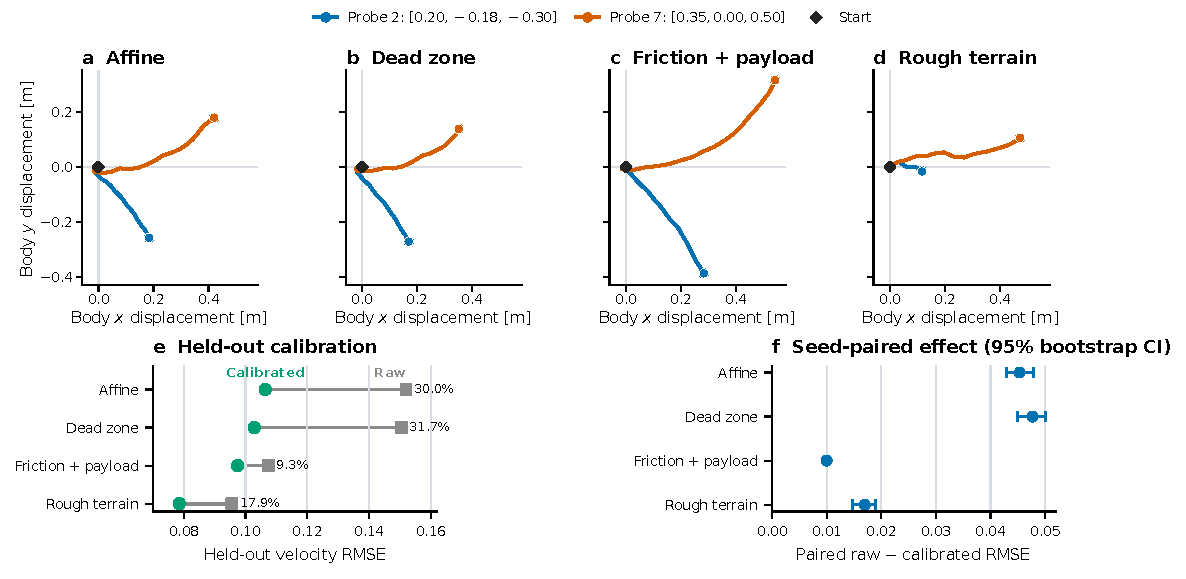
\includegraphics[width=\textwidth]{figures/p5_simulation_response.pdf}
  \caption{P5 registered simulation responses and closed-loop calibration.
  (a)--(d) Body-displacement trajectories for two validation probes at display
  seed 5301; diamonds and circles denote the common start and measured
  endpoints. (e) Raw and calibrated held-out velocity RMSE across 20 paired
  seeds; labels give relative reduction. (f) Seed-paired absolute improvement
  with 95\% 4,000-sample bootstrap intervals. The trajectories are qualitative
  examples; all inference uses the registered paired summaries.}
  \label{fig:p5scenes}
\end{figure*}

\begin{figure*}[t]
  \centering
  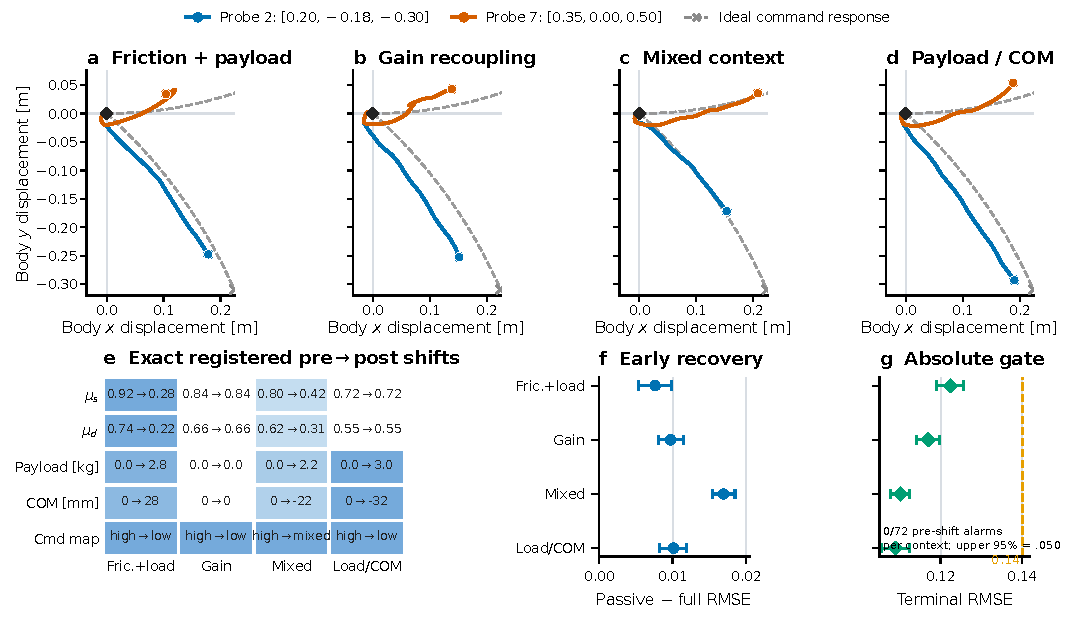
\includegraphics[width=\textwidth]{figures/p6_simulation_shift.pdf}
  \caption{P6 registered held-out shifts and active recovery. (a)--(d)
  Body-displacement trajectories for the same validation probes at display
  seed 10101. (e) Exact pre$\rightarrow$post static and dynamic friction,
  payload, fore--aft COM, and command-map settings; color intensity encodes
  within-row shift magnitude. (f) Full-method improvement over passive
  updating in the registered early window. (g) Full-method terminal RMSE and
  the frozen 0.14 gate. Error bars are paired 95\% 4,000-sample bootstrap
  intervals over 72 seeds per shift.}
  \label{fig:p6scenes}
\end{figure*}

\section{Results}

\begin{figure*}[t]
  \centering
  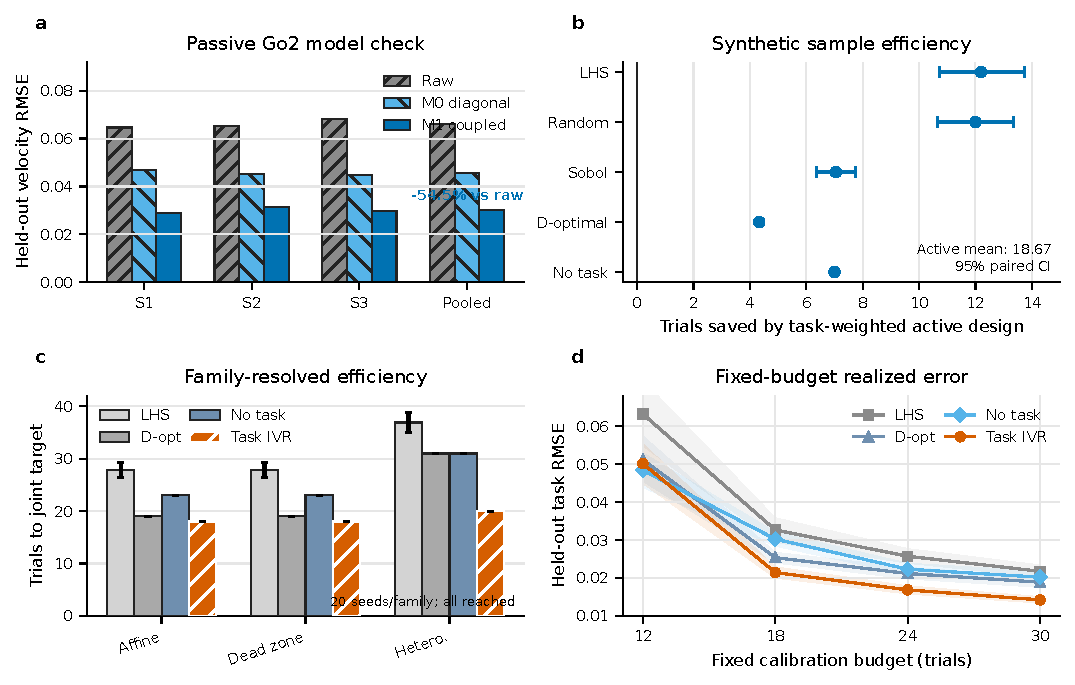
\includegraphics[width=\textwidth]{figures/calibration_evidence.pdf}
  \caption{Calibration evidence. (a) Passive real-Go2 held-out RMSE for raw,
  diagonal M0, and coupled M1 commands. (b) Paired trials saved by the
  task-weighted active method; bars are 95\% seed-bootstrap intervals for the
  paired difference.}
  \label{fig:calibration}
\end{figure*}

\subsection{Model Need and Calibration Efficiency}

Figure~\ref{fig:calibration}a shows a consistent held-out benefit from coupled
calibration on the passive Go2 data. Pooled RMSE falls from 0.06605 for raw
commands to 0.04563 for diagonal M0 and 0.03009 for coupled M1. M1 therefore
reduces error by 54.45\% versus raw commands and 34.07\% versus M0. The three
held-out-session M1 values are 0.02888, 0.03158, and 0.02974. The 30-trial LHS
M1 result is 3.33\% above the 122-trial dense reference (0.02912). These data
support a coupled correction for this robot and acquisition day; they do not
measure active hardware efficiency.

P3 isolates the acquisition rule (Fig.~\ref{fig:calibration}b). The full method
reaches the joint target in 18.67 trials, compared with 30.87 for LHS, 30.67
for random, 25.72 for Sobol, 23.00 for D-optimal, and 25.67 without task
weighting. Reductions are 39.52\%, 39.13\%, 27.41\%, 18.84\%, and 27.27\%,
respectively; all one-sided paired Wilcoxon tests give
$p=9.54\times10^{-7}$. The primary LHS comparison saves 12.20 trials with a
95\% interval of [10.73, 13.73]. Final active RMSE is 0.008462, 6.90\% above
the dense oracle's 0.007916, and 95\% predictive coverage is 94.14\%.

In closed-loop P5 simulation (Fig.~\ref{fig:p5scenes}e), raw-to-calibrated
RMSE is 0.15199 to 0.10635 for affine distortion, 0.15054 to 0.10282 for
dead-zone distortion, 0.10741 to 0.09742 for low friction plus payload, and
0.09554 to 0.07849 on rough terrain. Relative reductions span 9.30--31.70\%.
The corresponding paired absolute-improvement intervals are [0.04290, 0.04780],
[0.04495, 0.05002], [0.00981, 0.01017], and [0.01477, 0.01889]. All 20 paired
seeds improve in each scenario.

\subsection{Stopping, Safety, and Shift Recovery}

P4 records no premature stop across 60 trajectories. Median and p95 overshoot
after the oracle target are both two trials. The hard filter rejects 300/300
registered hazards and 0/20 safe controls; the runtime monitor catches all 160
fault injections with a maximum recorded detection latency of 0~ms. These are
software replay and fault-injection results, not physical safety certification.

Across the four P6 shifts, the full method improves early RMSE over passive
updating by 0.00761 for friction plus payload, 0.00974 for gain recoupling,
0.01691 for mixed context, and 0.01012 for payload/COM
(Fig.~\ref{fig:p6scenes}f). Their 95\% intervals are [0.00537, 0.00981], [0.00804,
0.01145], [0.01536, 0.01848], and [0.00825, 0.01194]. Detection succeeds in
72/72 seeds for three shifts and 71/72 for payload/COM; full recovery succeeds
in 72/72 for every shift. Worst p95 detection and recovery delays are four and
six trials. Full terminal RMSE ranges from 0.10898 to 0.12241, with every upper
interval endpoint below 0.126 (Fig.~\ref{fig:p6scenes}g). Passive updating can be
competitive at the terminal window, so the supported contrast is the
registered early-recovery effect.

\subsection{Navigation Consequence and Replication}

The first P7 strong confirmation did not pass. Full-method success was 68/72 on
one map and 50/72 on another, and some completion-time ratio interval upper
bounds reached 1.347. Trace inspection exposed a 10~Hz guard blind interval in
which base height could cross the hard limit between planner ticks. A 50~Hz
predictive height interlock was developed, frozen, and evaluated on six new
maps and seeds. No result from the failed confirmation or intervening pilots is
pooled with the replication.

\begin{figure*}[t]
  \centering
  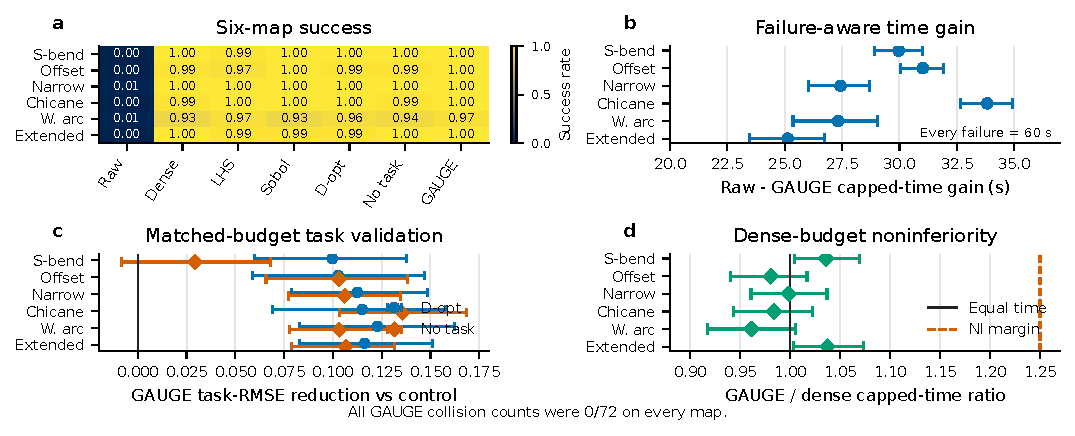
\includegraphics[width=\textwidth]{figures/navigation_results.pdf}
  \caption{P7 prospective simulator replication. (a) Success rate for six maps
  and seven methods (72 seeds/cell). (b) Paired completion-time gain of full
  calibration over raw control. (c) Full/dense time ratio with paired 95\%
  intervals; the registered noninferiority margin is 1.25. Every B8 collision
  count is 0/72.}
  \label{fig:navigation}
\end{figure*}

In the disjoint replication, B8 succeeds in 72/72 episodes on five maps and
70/72 on weighted arc (Fig.~\ref{fig:navigation}a); every B8 collision count is
zero. Paired B8-versus-raw completion-time gains have lower interval endpoints
from 23.453 to 32.675~s (Fig.~\ref{fig:navigation}b). The worst B8/dense mean
time-ratio interval upper bound is 1.0736, below the registered 1.25 margin, and
the worst ratio upper bound against any matched-budget control is 1.0901
(Fig.~\ref{fig:navigation}c). Because planner hashes and seeds are matched, the
comparison isolates command calibration within the frozen simulator pipeline.
It does not establish hardware navigation or sim-to-real transfer.

\section{Discussion and Limitations}

The experiments separate three questions that are often conflated. P1 asks
whether the exposed command interface needs coupled calibration. P3 asks
whether task weighting changes which trials are valuable. P7 asks whether a
calibration that looks accurate on held-out commands also preserves navigation
outcomes. The no-task and D-optimal controls show that the P3 gain is not merely
generic active learning, while the P7 protocol prevents validation RMSE from
rescuing a failed downstream endpoint.

The evidence has a clear hardware boundary. P1 is passive, same-day data from
one Go2 in one environment. P5--P7 use a pinned simulator and fixed policy. The
compact steady-response basis does not represent arbitrary history dependence,
gait switching, rapid transients, or shifts outside the registered families.
The planned P8 study must therefore execute active calibration on hardware,
apply gain/coupling, payload/COM, friction, and mixed shifts, and test navigation
on weighted-arc and offset-slalom courses. Until those data pass their frozen
gates, the present result is a simulator-validated calibration and recovery
architecture supported by passive hardware model evidence.

\section{Conclusion}

\method\ calibrates the high-level velocity interface of a fixed quadruped
controller by directing trials toward task-relevant predictive uncertainty.
The approach combines a coupled Bayesian model, exact IVR acquisition, hard
safety filtering, validated stopping, constrained inverse compensation, and
latched shift recovery. Passive Go2 measurements establish the need for a
coupled map; registered synthetic and Isaac Lab experiments establish sample
efficiency, early shift recovery, and downstream navigation under controlled
conditions. The remaining test is active real-robot execution of the same
frozen protocol.

\IEEEtriggeratref{10}
\bibliographystyle{IEEEtran}
\bibliography{references}

\end{document}
